\subsection{Sub-project for Keck Foundation support}

\begin{figure}[h!]
  \centering
  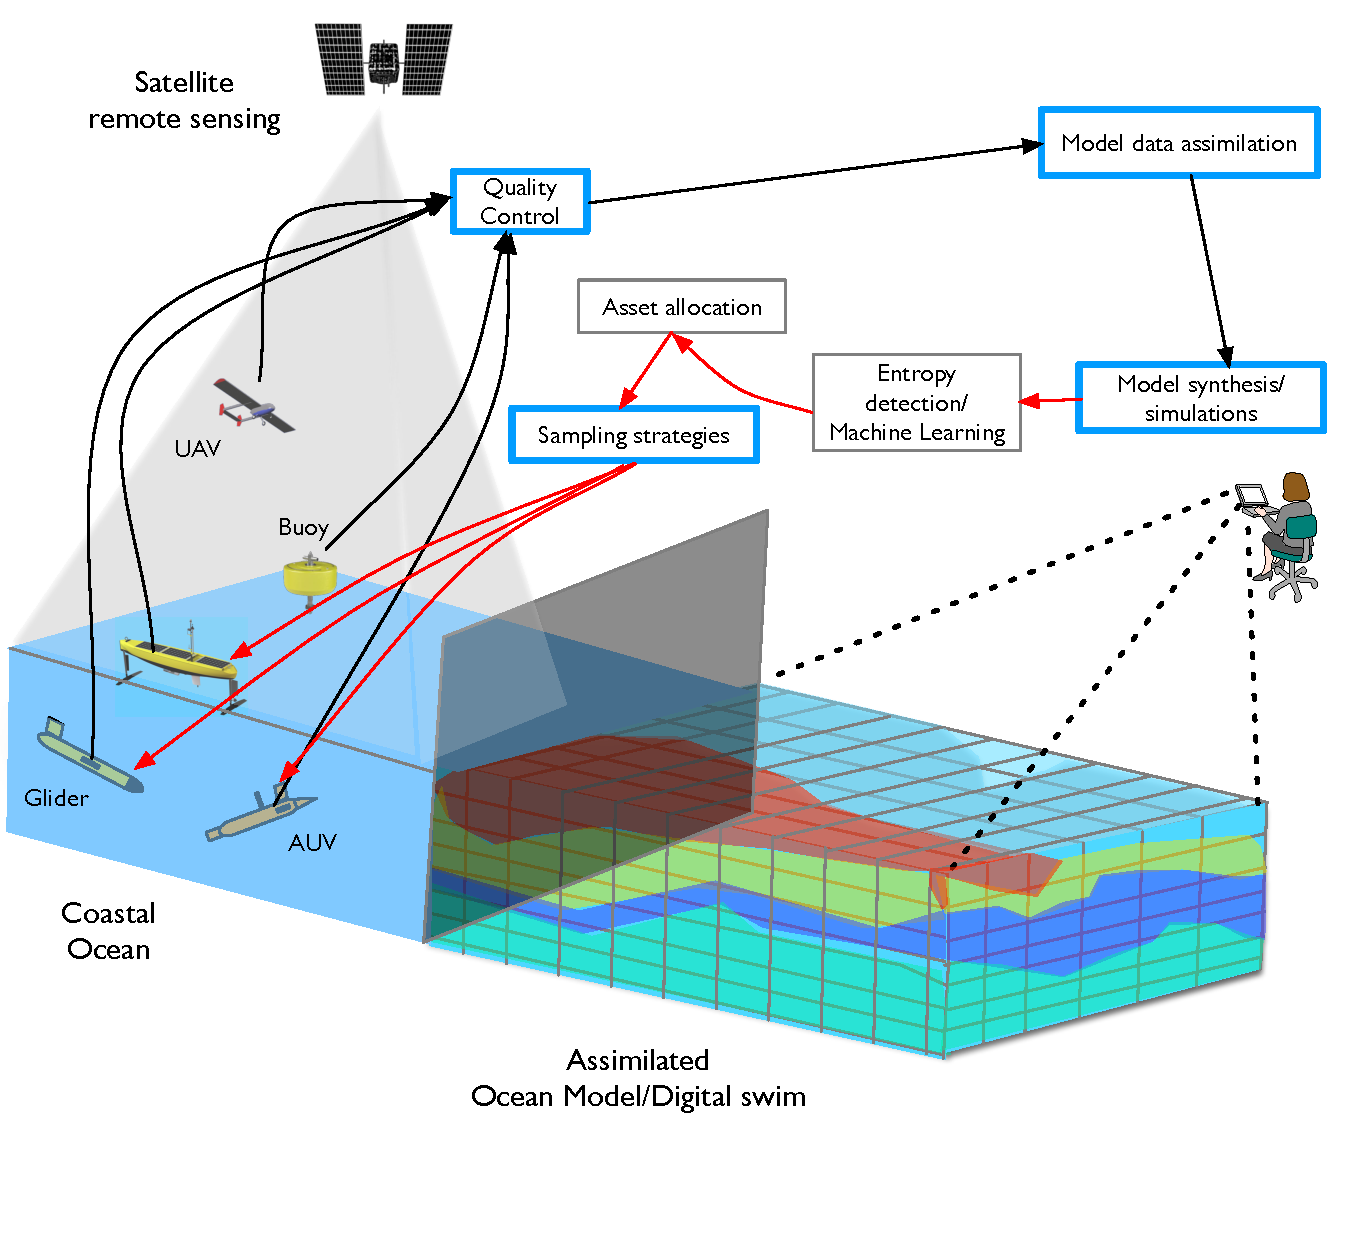
\includegraphics[scale=0.6]{fig/Audacious-pilot-block-diag-2.pdf}
  \caption{A representation of the technical tasks related to \proe. For
    the \kck the tasks related to model assimilation include portions of
    the boxes at the top of the figure in {\color{blue}{blue}}
    outline. Control aspects relate to using the assimilated ocean model
    to focus where and how autonomous platforms will make observation in
    the coastal ocean.}
    \label{fig:block-diag}
\end{figure}

In the first two years, \pro proposes to focus tasks to those related
to modeling, Bayesian model data assimilation, and planning and
control of autonomous robotic platforms. All individuals associated
with these efforts will be US-based.  Fig. \ref{fig:block-diag} shows
the associated tasks highlighted in {\color{blue}{blue}} and include:

\begin{description}

\item[Automated Data Pipeline, Quality Control \& Assimilation]
  Software and methods will be developed for rapid multi-platform data
  assimilation and learning, ensuring that the data is consistent with
  expectations of values. This will involve building a data pipeline
  and support infrastructure to ensure that any oceanographic sensor
  or robotic platform can feed data into our ocean model ready for
  assimilation. In addition, for this first phase, a data stream simulating the proposed small sat data (a "virtual constellation") will be constructed using data from existing US, European, and Japanese satellites. This task will require a software engineer with
  requisite skills related to data understanding, databases, ocean
  data formats.[SUGGEST DELETING THIS LAST SENTENCE - I.E NO MENTION OF FTES IN THIS SECTION]

\item[Ocean Data Modeling] To make model predictions, \pro will
  leverage off of the MIT Harvard Ocean Prediction System and its new
  MIT-MSEAS software\footnote{\url{http://mseas.mit.edu/HOPS/} and
    \url{http://mseas.mit.edu/software}}, focusing the model domains
  and processes to a region where a proposed field experiment can
  demonstrate the concepts in the 'real world'. The task will be to
  initialize the model with the geographical conditions of the
  selected region including the benthic topology and prime the model
  with remote sensing data adequate to initialize conditions for
  subsequent predictions.

\item[Prediction and Sampling Convergence] Using Bayesian predictive
  capabilities, \pro will pull together a methodology to narrow the
  prediction and sensing gap, between what is sensed in the real-world
  and what was predicted by our model. Strategies to close the
  expected gap will require the use of Machine Learning and
  Statistical techniques, to ensure that robotic platforms can observe
  in the most efficient, informative, and sustainable ways to bring
  about convergence, scientific understanding, and societal impact.

\item[Enhancing the Bio-geochemical model] Most models incorporate ocean
  dynamics and the physics related to water flow in the context of
  external forcings such as topology, wind, currents and fresh water
  inflow into the ocean. To make a realistic biological impact
  assessment of these dynamics, the variables associated with nutrients
  transport from the benthic as well as riverine environments, those
  derived from mixing and stirring in the upper water-column, as well as
  natural and anthropogenic changes need to be incorporated into the
  ocean model to produce plankton functional type responses. 

\item[Robotic Sampling Algorithms] To ``intelligently'' sample the upper
  water-column, marine robotic vehicles require the implementation of
  algorithms which can sample a wide range of coastal ocean phenomenon
  of interest including Harmful Algal Blooms, plumes, oil slicks and
  hypoxic zones. Using sensor data to craft algorithms embedded on AUVs,
  ASVs and potentially UAVs will require expertise in Statistical
  Sampling and autonomous decision-making and Control. \pro will ensure
  that the latest Sampling methods are embedded for computation on
  robotic vehicles.

\end{description}

\noindent
In addition to supporting the above tasks, \kck funding will help
coordinate work with our international partners ($\sim 10\%$ of
budget) and lay the foundation for demonstrating performance and
evaluating the operational skill of the proposed technologies. Some
support for instrumentation for use on robotic platform will also be
requested as part of this effort. A near-term goal would be to iterate
between software development and field implementation efforts at the
Univ. of Porto, Portugal; this collaboration allows for leveraing the
substantial in-situ robotic assets and expertise present there.  Doing
so would allow the team to position \pro to obtain other support to
fulfill the ambition of the entire project proposed in this document.

Importantly, we hope to demonstrate the preliminary capabilities of \pro in the field by the end of two years.  One possibility is the New York Bight region, an Urban Sea experiencing high human impact.  The New York Bight has had a history of pollution related hypoxic events in the past and ongoing concerns related to ocean pollution (excess nutrients and plastics), harmful algal blooms, storm surges and ocean
exploitation (fisheries, shipping, tourism, and plans to construct offshore wind farms). We have
capabilities to involve local government entities, non-profits,
high-school students, and museums and press, including a strong
emphasis on diversity, equity and inclusion efforts related to the
sustainable utilization and protection of our coastal regions.

